
\chapter{自动语音识别}
\label{chap:intro}
\section{自动语音识别框架}
\label{chap:intro-asr}


这一章我们将主要介绍在大词汇连续语音识别(LVCSR)中一些基本内容,图~\ref{fig:asr}中所描绘的几个部分都会在本章描述。这主要包括:特征提取前端、子词单元的挑选、隐马尔可夫、解码搜索、语言模型等内容。

\subsection{特征提取}
\label{sec:feat_extra}
语音信号原始形态是  一种连续的波形语音,为了能进行 更有效的识别,通常我们会先将连续的波形转换为一个离散的实数序列向量$\mathbf{O}=\left[ \mathbf{o}_1, ..., \mathbf{o}_T \right]$。每一个向量都是压缩后的语音变化的一种表示。这些向量也被称为 特征向量或者观测特征向量。语音信号是一个准平稳信号,所以我们首先需将其切成若干重叠离散片段,通常是将一个25毫秒长窗口以10毫秒 的间隔向后滑动,通过此方法提取出的 一个片段被称为一帧。通常会利用汉明(Hamming)窗或者汉宁(Hanning)窗来进行平滑,为减小边界效应,继而利用快速傅立叶变换将其从时域特征转变为频域特征。在得到频域上的复数特征后,通过利用不同的后处理方法可以得到不同特征:典型的有感知线性预测系数(Perceptual Linear Prediction, PLP)~\cite{hermansky1990perceptual}和梅尔倒谱系数(Mel-Frequency Cepstral Coefficients, MFCC)~\cite{davis1980comparison}。近来,由于深度神经网络拥有更强大的建模能力,研究者发现保留梅尔滤波器输出中维度之间的相关性的滤波器组特征(Filter Bank Feature, FBANK)~\cite{seide2011feature}更适合于深度神经网络利用,接下来将对这三种特征进行详细介绍:
\begin{itemize}
    \item 滤波器组特征 \\
    1. 在得到了频率谱的复数特征后,相位信息通常会被丢弃,而仅仅只有复数特征的幅度部分会留下,接着频率轴会通过梅尔频率缩放公式进行调整,最终我们可以得到一个缩放后的幅频域特征:
    \begin{equation}
        \text{Mel}(f)=2595 \log_{10}(1+\frac{f}{500}) 
    \end{equation}
    2. 接着,不同的滤波器含有不同的滤波增益,一组三角滤波器将被用于降采样这一幅频域特征。最终一个滤波器的 输出为幅度特征乘上滤波器中对应频率增益的自然对数求和。通常而言,对于8K采样率的语音会利用36组滤波器,对于16K的语音会利用40组。
    \item 梅尔倒谱系数 \\
    梅尔倒谱系数特征在FBANK特征基础上进一步利用离散余弦变换来计算倒谱系数以减少滤波器的组之间相关性。通常利用12个的倒谱系数加上归一化后功率自然对数组成一个13维特征的向量。
    \item 感知线性预测系数 \\
    1. 感知线性预测系数是另外一种倒谱的特征,它利用Bark公式来缩放频率的轴:
    \begin{equation}
        \text{Bark}(f)=6\log \left( \left( \frac{f}{600}+1 \right)^{0.5}+\frac{f}{600} \right)
    \end{equation}
    2. 接着它利用功率谱(幅度的平方)来提取感知线性的特征,之后该功率谱会与一个临界的频带滤波器进行卷积并且通过等响度的曲线进行预加重。\\
    3. 最后通过利用线性预测分析来获得倒谱的系数。
\end{itemize}
在提取了原始声学的特征之后,通常会利用一些后处理方法:
\begin{itemize}
    \item 动态特征~\cite{furui1986speaker}:一阶动态特征的计算公式如下
    \begin{equation}
        \Delta_{\mathbf{o}_t}=\frac{\sum_{k=1}^K k(\mathbf{o}_{t+k}-\mathbf{o}_{t-k})}{2\sum_{k=1}^K{k^2}}
    \end{equation}
    其中$K$是动态特征计算窗的大小,通常设置为2。二阶动态特征是最为常用的,其计算方法和一阶一致,只不过将$\mathbf{o}_t$替换为$\Delta_{\mathbf{o}_t}$。在利用了动态特征后,特征的不同维度之间产生了相关性,这与后面一些声学模型建模方法中做出特征各维度之间独立性的假设产生了冲突。因此,为消除特征各维度之间相关性,通常会利用线性投影方法,如异方差线性判别分析(Heteroscedastic Linear Discriminant Analysis, HLDA)~\cite{kumar1998heteroscedastic}等。
    \item 特征正则化: 特征正则化目标是消除声学特征中的非语音变化,同时它也能将特征的值域范围进行归一化,这一操作对于深度神经网络来说特别重要。传统的正则化方法包括倒谱均值归一化(Cepstral mean normalisation, CMN)~\cite{atal1974effectiveness}, 倒谱方差归一化(Cepstral variance normalisation, CVN)\cite{woodland1995development}以及声道长度归一化(Vocal tract length normalisation, VTLN)~\cite{lee1996speaker}。其中倒谱均值归一化(CMN)将输入特征向量的每个维度的均值归一化为0,倒谱方差归一化(CVN)将输入特征向量的每个维度的方差归一化为1。归一化可以运用在不同层面-包括说话人层面及句子层面。声道长度归一化(VTLN)被用来减少声学特征中的说话人变化,它的原理是将来自于同一个说话人特征频率轴进行同样大小缩放。
\end{itemize}

\subsection{声学模型}
声学模型的作用是计算一个候选词序列$\mathbf{w}$生成出观测到的特征向量序列$\mathbf{O}$概率。它从概率论角度提供了给定词标注之后语音信号生成的过程。在传统GMM-HMM声学模型中,HMM建模了语音的序列性,GMM建模了特征向量生成的概率。在最新的基于深度神经网络的声学模型中,深度神经网络被用来计算特征向量生成概率。 GMM-HMM将在章节\ref{sec:hmm}中详细介绍,DNN-HMM将在章节\ref{sec:dnn_hmm}中详细介绍。声学模型是语音识别系统中最核心部件之一,也是本论文研究重点。

\subsubsection{隐马尔可夫模型 (HMM)}
\label{sec:hmm}
隐马尔可夫模型是一个统计学中生成模型,在语音识别领域获得了重大成功。在隐马尔可夫模型中,一个特定声学的单元,如一个单词或一个音素将被建模为一个有限状态机,而我们所观测到特征序列则是由该音频所对应的词序列连接成的有限状态机生成的。在每个时间单元,状态将以一个给定的概率分布发生转变:跳转到下一个状态或保持在当前状态。变换完成后,将由另一个概率函数生成一个特征向量。一个拥有三个输出状态的从左到右隐马尔可夫模型如图\ref{fig:hmm}所示,其中状态1和5是进入状态和退出状态,它们并不输出观测特征向量。这一结构是语音识别中最常用结构。

\begin{figure}[!htp]
  \centering
    \captionstyle{\centering}
    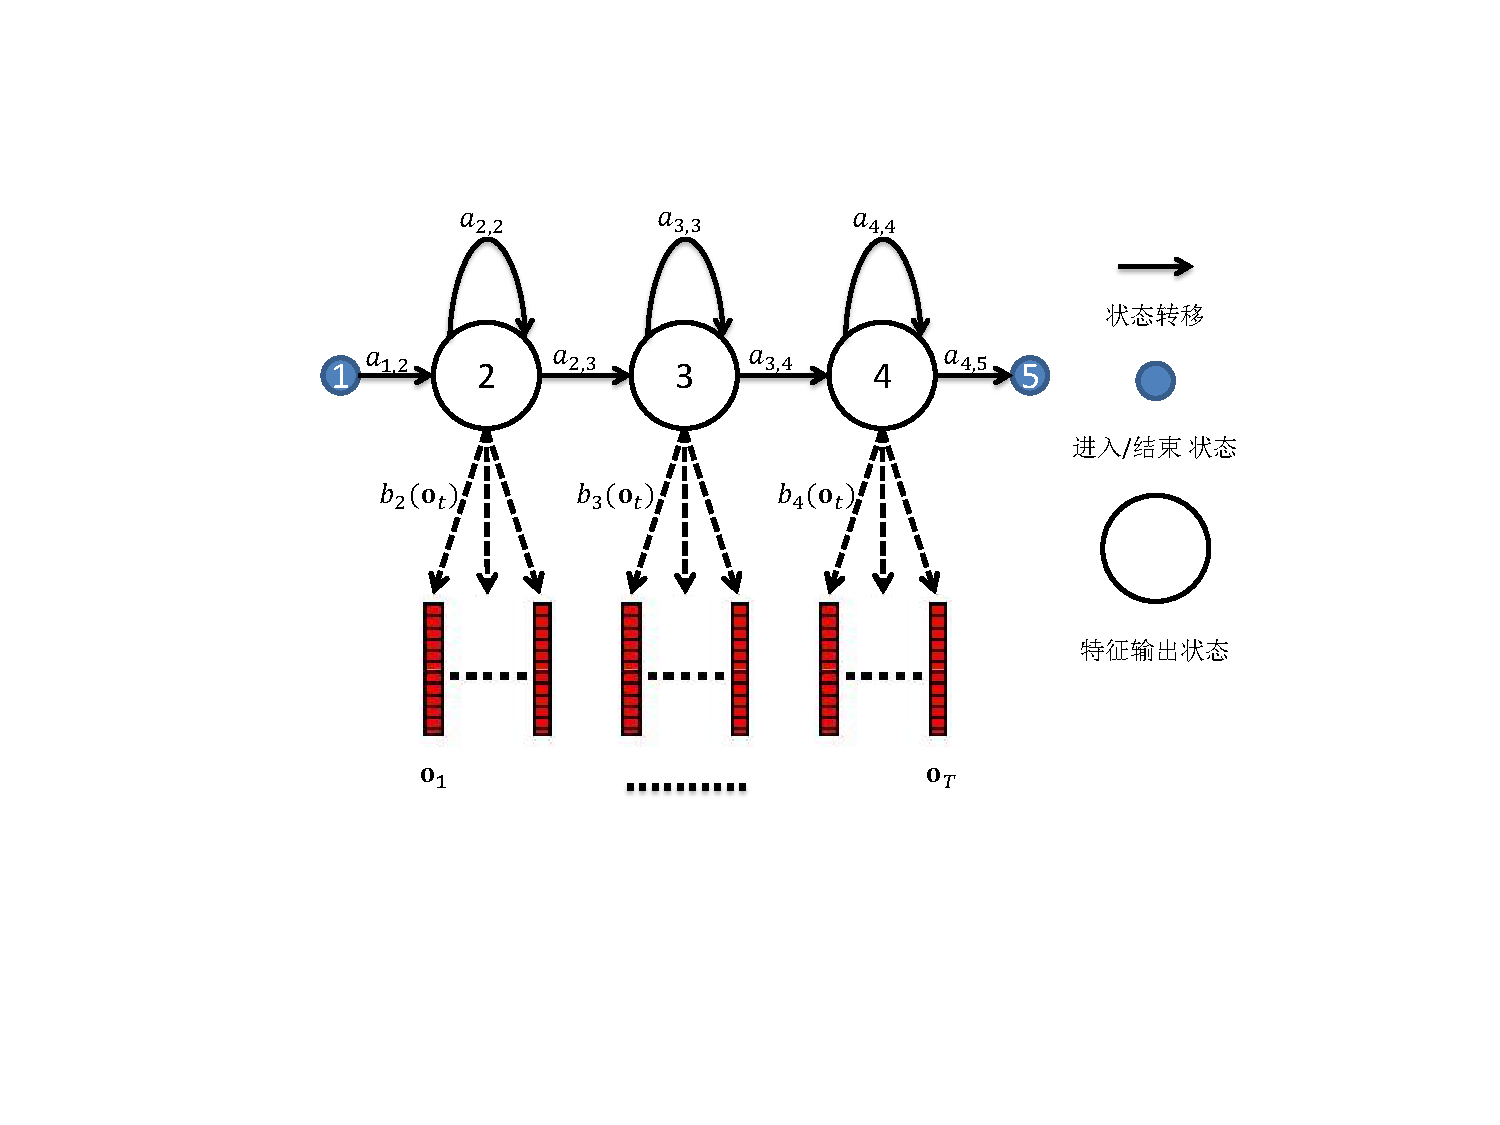
\includegraphics[trim = 3cm 5cm 4cm 3cm, clip=true, width=.7\textwidth]{figure/hmm.pdf}
    \bicaption[fig:hmm]{}{隐马尔可夫模型}{Fig}{Hidden Markov Model}
\end{figure}

令$\mathbf{O}=[\mathbf{o}_1, ..., \mathbf{o}_T]$为由一个声学单元生成的特征向量序列,其中$\mathbf{o}_t$是一个第$t$时刻的$D$维的语音特征向量,$T$是语音序列的总帧数。声学特征序列的生成过程如下面所示:
\begin{enumerate}
    \item 在第0时刻从状态1开始
    \item 在时刻$t$($0 \le t \le T-1$)。假设当前处于状态$i$,以概率$a_{i,i+1}$跳转到状态i+1或者以概率$a_{i,i}$停留在当前状态。
    \item 假设跳转完后处于状态$j$,若此时处在输出状态,则以$b_j(\mathbf{o}_t)$的概率输出声学向量$\mathbf{o}_t$。
    \item 重复2直至到达状态5
\end{enumerate}

这样我们可以利用一个状态序列来描述语音特征的输出过程$\mathbf{s}=[s_1, ..., s_T]$。而现实中我们只能观察到由状态输出语音特征序列,状态序列$\mathbf{s}$是隐藏的,这也是该模型被称为隐马尔可夫模型原因。一个隐马尔可夫模型通常包含如下参数:
\begin{itemize}
    \item $\pi$ 初始状态分布: \\
    令$s_t$表示在时刻t时所处状态,那么$\pi_i = P(s_0=i), \sum_{i=1}^N \pi_i = 1, \pi_i \ge 0$,其中$N$是总状态数。在拥有进入状态隐马尔可夫模型中,通常$\pi_1=1$。
    \item 状态转移概率矩阵$\mathbf{A}$: \\
    $a_{i,j}=P(s_{t+1}=j|s_t=i)$,在最常用5状态隐马尔可夫模型中,通常只有$a_{i,i}和a_{i,i+1}$不为0
    \item 状态输出概率分布$\mathbf{B}$: \\
    每个特征输出状态$i$都有一个概率分布来输出一帧声学特征,$b_i(\mathbf{o}_t)=p(\mathbf{o}_t|s_t=i)$
\end{itemize}

\subsubsection{混合高斯模型 (GMM)}
在传统的GMM-HMM中,状态输出概率$b_i(\mathbf{o}_t)$通常由一个混合高斯模型来建模。概率计算公式如下:
\begin{equation}
    b_i(\mathbf{o}_t)=\sum_{m=1}^{M_i}c^m_{i}\mathcal{N}(\mathbf{o}_t;\bm{\mu}^m_{i},\bm{\Sigma}^m_{i})
\end{equation}
其中$M_i$是属于第$i$个状态混合高斯模型含有的高斯成分个数,$c^m_{i}$是混合权重,满足$c^m_{i} \ge 0, \sum_{m=1}^{M_i} c^m_{i}=1$。$\mathcal{N}(\mathbf{o}_t;\bm{\mu}^m_{i},\bm{\Sigma}^m_{i})$是均值为$\bm{\mu}^m_{i}$,协方差矩阵为$\bm{\Sigma}^m_{i}$多变量高斯分布。
\begin{equation}
    \mathcal{N}(\mathbf{o};\bm{\mu},\bm{\Sigma})=(2\pi)^{-\frac{D}{2}}{|\bm{\Sigma}|}^{-\frac{1}{2}}e^{-\frac{1}{2}(\mathbf{o}-\bm{\mu})^{\top}\bm{\Sigma}^{-1}(\mathbf{o}-\bm{\mu})}
\end{equation}

\subsubsection{HMM的似然计算}
\label{sec:calc_like}
在定义好了HMM中分布之后,我们就可以计算隐马尔可夫模型的似然。似然计算目标是给定一个语音特征向量序列和一个隐马尔可夫模型,计算该模型生成给定的语音特征向量序列概率,即计算$p(\mathbf{O}|\mathbf{w},\mathcal{M})$,其中$\mathbf{O}$为观测到的语音特征向量序列,$\mathbf{w}$为对应文本标注,$\mathcal{M}=\{\pi, \mathbf{A}, \mathbf{B}\}$是所有模型参数。由于状态序列$\mathbf{s}$是隐藏,因而需要枚举所有可能的状态序列并求其期望,即:
\begin{eqnarray}
p(\mathbf{O}|\mathbf{w},\mathcal{M}) &=& \sum_{s}p(\mathbf{O},\mathbf{s}|\mathbf{w},\mathcal{M}) \\
&=& \sum_{\mathbf{s}} P(\mathbf{s}|\mathbf{w},\mathcal{M})p(\mathbf{O}|\mathbf{s},\mathcal{M}) \\
&=& \sum_{\mathbf{s}} a_{s_0, s_1}\prod_{t=1}^T a_{s_{t-1}, s_t}b_{s_t}(\mathbf{o}_t)
\end{eqnarray}
以上只考虑了单个隐马尔可夫模型似然计算。对于连续语音识别或利用子单词的声学单元,语音序列将对应一个模型序列。各个单词或者子单词单元之间准确时间边界是未知的,而解决方法则是扩展单隐马尔可夫模型,将若干个单独隐马尔可夫模型连接起来组成组合隐马尔可夫模型。

似然计算是利用和训练隐马尔可夫模型时需要考虑的最核心问题,直接枚举所有状态序列复杂度无疑是很高的。这一概率可以利用前向-后向算法快速计算,该算法也被称作鲍姆威尔士算法~\cite{baum1967inequality}(Baum-Welsh algorithm)。前向-后向算法通过利用动态规划思想,只需要$O(N^2T)$时间复杂度即可以计算出该概率,其中$N$是总状态数,$T$是总帧数。

定义前向概率$\alpha_i(t)$为到t时刻为止,且第t时刻所处状态为$i$,观测到特征序列$\left( \mathbf{o}_1, \dots, \mathbf{o}_t \right)$的概率。
\begin{equation}
\alpha_i(t)=p(\mathbf{o}_1, \dots, \mathbf{o}_t,s_t=i|\mathbf{w}, \mathcal{M})
\end{equation}
前向概率可以通过递归快速计算,对于$1<i<N, 0<t<=T$
\begin{equation}
\alpha_i(t)=(\sum_{j=1}^{N-1}\alpha_j(t-1)a_{j,i})b_i(\mathbf{o}_t)
\end{equation}
边界条件为:
\begin{eqnarray}
\alpha_i(t)=
\begin{cases}
1& i=1,t=0 \\
0& i \ne 1,t=0 \\
\sum_{j=2}^{N-1}\alpha_i(T)a_{j,N}& i=N, t=T+1
\end{cases}
\end{eqnarray}
对于常用于语音识别五状态HMM而言,因为转移只存在于相邻两个状态之间,所以时间复杂度减少为$O(NT)$。

同样我们可以定义后向概率$\beta_i(t)$为从第t时刻开始,且第t时刻所处状态为$i$的概率,观测到特征序列$\left( \mathbf{o}_{t+1}, \dots, \mathbf{o}_T \right)$概率。
\begin{equation}
\beta_i(t)=p(\mathbf{o}_{t+1},...,\mathbf{o}_T|s_t=i, \mathbf{w}, \mathcal{M})
\end{equation}
后向概率也可以通过递归快速计算,对于$1<i<N, 0<t<T$
\begin{equation}
\beta_i(t)=\sum_{j=1}^{N} a_{i,j} b_j(\mathbf{o}_{t+1}) \beta_j(t+1)
\end{equation}
边界条件为:
\begin{eqnarray}
\beta_i(t)=
\begin{cases}
a_{i,N} & t=T \\
\sum_{j=2}^{N-1} a_{1,j} b_j(\mathbf{o}_{1}) \beta_j(1) & i=1, t=0
\end{cases}
\end{eqnarray}
计算完前向概率和后向概率之后,可以很容易得到似然的公式为:
\begin{equation}
    p(\mathbf{O}|\mathbf{w}, \mathcal{M})=\alpha_N(T+1)=\beta_1(0)
\end{equation}

\subsubsection{最大似然估计}
训练GMM-HMM通常采用最大似然估计(Maximal Likelihood Estimation, MLE)准则。令$\mathcal{M}= \lbrace \{ a_{i,j}, 1 \le i,j \le N \}, \{ c^m, \bm{\mu}^m, \bm{\Sigma}^m, 1 \le m \le M \} \rbrace$为GMM-HMM中所有参数。其中$N,M$分别为总状态数和总高斯成分数。优化准则即为:
\begin{equation}
    \hat{\mathcal{M}}_{\text{MLE}} = \arg \max_{\mathcal{M}}\log p(\mathbf{O}|\mathbf{w}, \mathcal{M}) 
\end{equation}
由于存在隐藏变量,直接优化上述公式是很困难的,利用最大期望算法(Expectation-Maximization, EM)~\cite{dempster1977maximum}可对此进行优化。EM算法被广泛运用于含有隐变量统计学模型中,它基本思想是引入一个辅助函数作为log似然下界,通过不断迭代优化辅助函数来优化log似然函数。对于隐马尔可夫模型而言,辅助函数定义为:
\begin{eqnarray}
\mathcal{Q}_{\text{MLE}}(\mathcal{M}_{k+1};\hat{\mathcal{M}_{k}}) &=& \sum_{\mathbf{s}} P(\mathbf{s}|\mathbf{O},\mathbf{w}, \hat{\mathcal{M}}_k) \log p(\mathbf{O}, \mathbf{s}|\mathbf{w}, \mathcal{M}_{k+1}) \\
&=& \sum_{t,i} \gamma_i(t)\log b_i(\mathbf{o}_t) + \sum_{t,i,j}\xi_{ij}\log a_{i,j}
\end{eqnarray}
其中$\hat{\mathcal{M}}_k$是第$k$轮迭代计算出最优参数,
\begin{eqnarray}
\gamma_i(t)&=&P(s_t=i|\mathbf{O},\mathbf{w},\hat{\mathcal{M}}_k) \\
\xi_{ij}(t)&=&P(s_{t-1}=i,s_t=j|\mathbf{O},\mathbf{w},\hat{\mathcal{M}}_k)
\end{eqnarray}
EM算法是一个迭代的优化过程,其优化步骤如下:
\begin{enumerate}
    \item 初始化模型$\hat{\mathcal{M}}_0$
    \item 设当前迭代到第$k$轮,已经训练好模型参数$\hat{\mathcal{M}}_k$
    \item 利用$\hat{\mathcal{M}}_k$估计后验概率$\gamma_i(t)$, $\xi_{ij}(t)$。这两个概率可以由上一节提到的前向后向算法计算$\alpha,\beta$快速获得:
    \begin{eqnarray}
    \gamma_i(t)&=&\frac{\alpha_i(t)\beta_i(t)}{p(\mathbf{O}|\mathbf{w}, \hat{\mathcal{M}}_k)} \\
    \xi_{ij}(t)&=&\frac{\alpha_i(t-1)a_{i,j}b_j(\mathbf{o}_t)\beta_j(t)}{p(\mathbf{O}|\mathbf{w}, \hat{\mathcal{M}}_k)}
    \end{eqnarray}
    \item 利用最大似然估计$\hat{\mathcal{M}}_{k+1}$
    \begin{equation}
        \hat{\mathcal{M}}_{k+1} = \arg \max_{\mathcal{M}} \sum_{t,i} \gamma_i(t)\log b_i(\mathbf{o}_t) + \sum_{t,i,j}\xi_{ij}\log a_{i,j}
    \end{equation}
    \item 转移概率更新为:
    \begin{equation}
        \hat{a}_{i,j}=\frac{\sum_{t=1}^T \xi_{i,j}(t)}{\sum_{t=0}^{T+1} \gamma_i(t)}
    \end{equation}
    \item 当利用GMM作为状态输出概率时,高斯成分的索引可以被视为一个特殊隐子状态,转移概率是各成分的权重乘以状态转移概率。因此可以求得各个高斯成分后验占用率:
    \begin{equation}
        \gamma^m_j(t)=\frac{\sum_{i=2}^{N-1}\alpha_i(t-1)a_{i,j}c^m_{j}\mathcal{N}(\mathbf{o}; \bm{\mu}^m_j, \bm{\Sigma}^m_j)\beta_j(t)}{p(\mathbf{O}|\mathbf{w}, \hat{\mathcal{M}}_k)}   
    \end{equation}
    这里$\gamma^m_j(t)$表示状态$j$的第$m$个高斯成分在第$t$包含后验占有量。
    \item GMM的参数更新为:
    \begin{eqnarray}
        \hat{c}^m_j &=& \frac{\sum_{t=1}^T \gamma^m_j(t)}{\sum_{m,t} \gamma^m_j(t)} \\
        \hat{\bm{\mu}}^m_j &=& \frac{\sum_{t=1}^T \gamma^m_j(t) \mathbf{o}_t}{\sum_{t=1}^T \gamma^m_j(t)} \\
        \hat{\bm{\Sigma}}^m_j &=& {\tt diag} \left( \frac{\sum_{t=1}^T \gamma^m_j(t) (\mathbf{o}_t-\hat{\bm{\mu}}^m_j)(\mathbf{o}_t-\hat{\bm{\mu}}^m_j)^{\top}}{\sum_{t=1}^T \gamma^m_j(t)} \right)
    \end{eqnarray}
    在公式中,我们只估计了协方差矩阵对角元素。由于在大词汇连续语音识别任务中通常需要利用大量高斯成分,在此基础上若利用满秩矩阵将对计算和存储资源需求巨大,因而对于每个高斯成分,通常只利用对角矩阵。
    \item 重复2直到收敛
\end{enumerate}
虽然利用最大似然估计GMM-HMM已获得了巨大成功,然而只有在拥有充足数据量和正确的模型假设前提下它才是合适优化准则。现实中,由于在HMM模型中存在马尔可夫和条件独立性两个假设,并不符合真正语音生成过程,因此利用最大似然估计来最优化HMM将无法估计出最合适的参数。其中一个解决方案就是利用序列鉴别性训练准则~\cite{bahl1986maximum,schluter2001comparison,chou1993minimum,goel2000minimum,juang1997minimum,povey2005discriminative,povey2001improved}

\subsubsection{序列鉴别性训练}
在基于最大似然估计中,优化目标是给定标注生成语音特征向量序列的似然。鉴别性训练与之不同处在于:鉴别性训练优化目标为最大化给定语音特征向量序列所对应文本标注的后验概率,即最大化$P(\mathbf{w}_{\text{ref}}|\mathbf{O})$。这样相当于直接将语音识别评判准则引入优化目标之中。目前最先进的语音识别系统中都利用了序列鉴别性准则。这章将简单地介绍其中两种:最大互信息(Maximum Mutual Information, MMI)和最小贝叶斯风险(Minimum Bayes' Risk, MBR)
\begin{itemize}
    \item 最大互信息 \\
    最大互信息准则在后验概率$P(\mathbf{w}_{\text{ref}}|\mathbf{O})$基础上增加一个经验缩放$\kappa$\footnote{它的作用是为了使不太可能假设对准则有所贡献,并使准则更加平滑可区分,通常等于识别中利用的语言模型缩放系数倒数},它的优化目标如下:
    \begin{equation}
        \mathcal{F}_{\text{MMI}}(\mathcal{M})=\frac{p^{\kappa}(\mathbf{O}|\mathbf{w}_{\text{ref}},\mathcal{M})P(\mathbf{w}_{\text{ref}})}{\sum_{\mathbf{w}}p^{\kappa}(\mathbf{O}|\mathbf{w},\mathcal{M})P(\mathbf{w})}
    \end{equation}
    这里$\mathbf{w}_{\text{ref}}$是语音特征向量序列对应标注,$\mathbf{w}$是所有可能的标注序列,包括正确标注和错误标注。虽然理论上$\mathbf{w}$应该包括所有可能词序列,实际上通常只考虑最具有混淆性标注。它通常由在训练数据上解码生成N-Best列表或者词图构成。
    \item 最小贝叶斯风险 \\
    最小贝叶斯风险准则目标在最小化期望损失,即
    \begin{equation}
        \mathcal{F}_{\text{MBR}}(\mathcal{M})=\sum_{\mathbf{w}}P(\mathbf{w}|\mathbf{O};\mathcal{M})L(\mathbf{w},\mathbf{w}_{\text{ref}})
    \end{equation}
    这里$L(\mathbf{w},\mathbf{w}_{\text{ref}})$是标注与候选的标注之间损失函数,通常包含句子层,单词层和音素层。
    \begin{itemize}
        \item 句子层:这一准则希望最小化句子层的错误
        \begin{eqnarray}
            L(\mathbf{w},\mathbf{w}_{\text{ref}})=
            \begin{cases}
                1& \mathbf{w} \ne \mathbf{w}_{\text{ref}} \\
                0& \mathbf{w} = \mathbf{w}_{\text{ref}}
            \end{cases}
        \end{eqnarray}
        \item 损失函数也可以定义在词层面(最小词错误)和音素层面(最小音素错误)。比如在最小词错误中,$L(\mathbf{w},\mathbf{w}_{\text{ref}})$为两个词序列之间编辑距离,即词错误数。最小音素错误在最先进语音识别系统中利用非常广泛~\cite{povey2005discriminative}
    \end{itemize}
\end{itemize}

\subsubsection{声学单元和参数绑定}
当进行小词汇语音识别时,如识别数字时通常可以用隐马尔可夫模型直接建模独立的单词。然而当词汇数量从中等词汇上涨到大词汇(>10000)时,利用隐马尔可夫模型来建模每一个词汇变成了不可能事情。一个广泛利用的解决该问题方法为建模子词单元。

音素是一个被广泛利用的子词单元,它是语音中最小声学元素。利用音素的好处是存在将每个词转换为音素标准,这样每个词能很容易的被分解成各个音素。在音素上建模的模型被称作音素模型,音素数目一般远远小于待识别词的个数。在当前最先进大词汇连续语音识别系统里,通常利用46个音素。

利用音素能更容易的获得足够数据以训练出更具有鲁棒性的模型参数。需要注意是当利用音素来建模时,需要提供一个字典用于将单词序列映射成子词单元序列,然后才能在子词单元的层面进行识别和运算。在识别最后,还需要将子词单元序列转换回单词序列。

目前有两种被广泛利用音素集合。一种是单音素,也称为上下文无关音素;另一种则是上下文相关音素。由于协同发音现象的影响,当前音素发音和前一个、后一个音素之间具有很强的相关性,所以在许多识别任务里,仅仅利用单音素效果不是很好。为了建模协同发音现象,目前最先进语音识别系统利用的是上下文相关音素,其中三音速利用最为广泛,它将当前音素的前一个和后一个音素同时建模。

比如,以one来说,它对应三音素序列即扩展为one=\{sil−w−ah, w-ah-n, ah-n-sil\}。虽然利用更多的上下文信息可以建立更复杂的音素模型,如五音素~\cite{hain2005automatic}(quin-phones),但三音素依然是目前利用最广泛音素模型。根据是否考虑单词间的边界,三音素模型可以继续细分为跨单词三音素和单词内三音素。跨单词三音素允许三音素的扩展跨越单词:在两个单词边界,当前音素的前一个和后一个音素分别是上一个单词的最后一个音素和下一个单词第一个音素。词内三音素则相反,音素只能在单词的内部进行扩展。因此,在每个单词开头和结尾,是一个双音素。跨单词三音素在大规模词汇连续语音识别系统里效果更好~\cite{woodland1994large}。

利用三音素后,声学单元个数将变得巨大。当利用46个单音素时,所有可能的三音素个数达到了$46^3=97336$,这一数字甚至超过了词表大小,不可能有充足数据能训练如此大的模型。目前一个通用解决该问题的方法是利用参数共享~\cite{young1993use, young1994tree}。它基本思想是将一些参数绑定在一起。参数共享可以存在于各个层面,包括音素,状态,高斯等。由于利用最广泛的是在状态共享层面,因而也被称为状态聚类。在利用状态聚类时,来自同一组的状态将共享状态输出分布,每一个实际状态输出分布被称为一个语素(senone),如图\ref{fig:state-tying}所示。
\begin{figure}[!htp]
  \centering
    \captionstyle{\centering}
    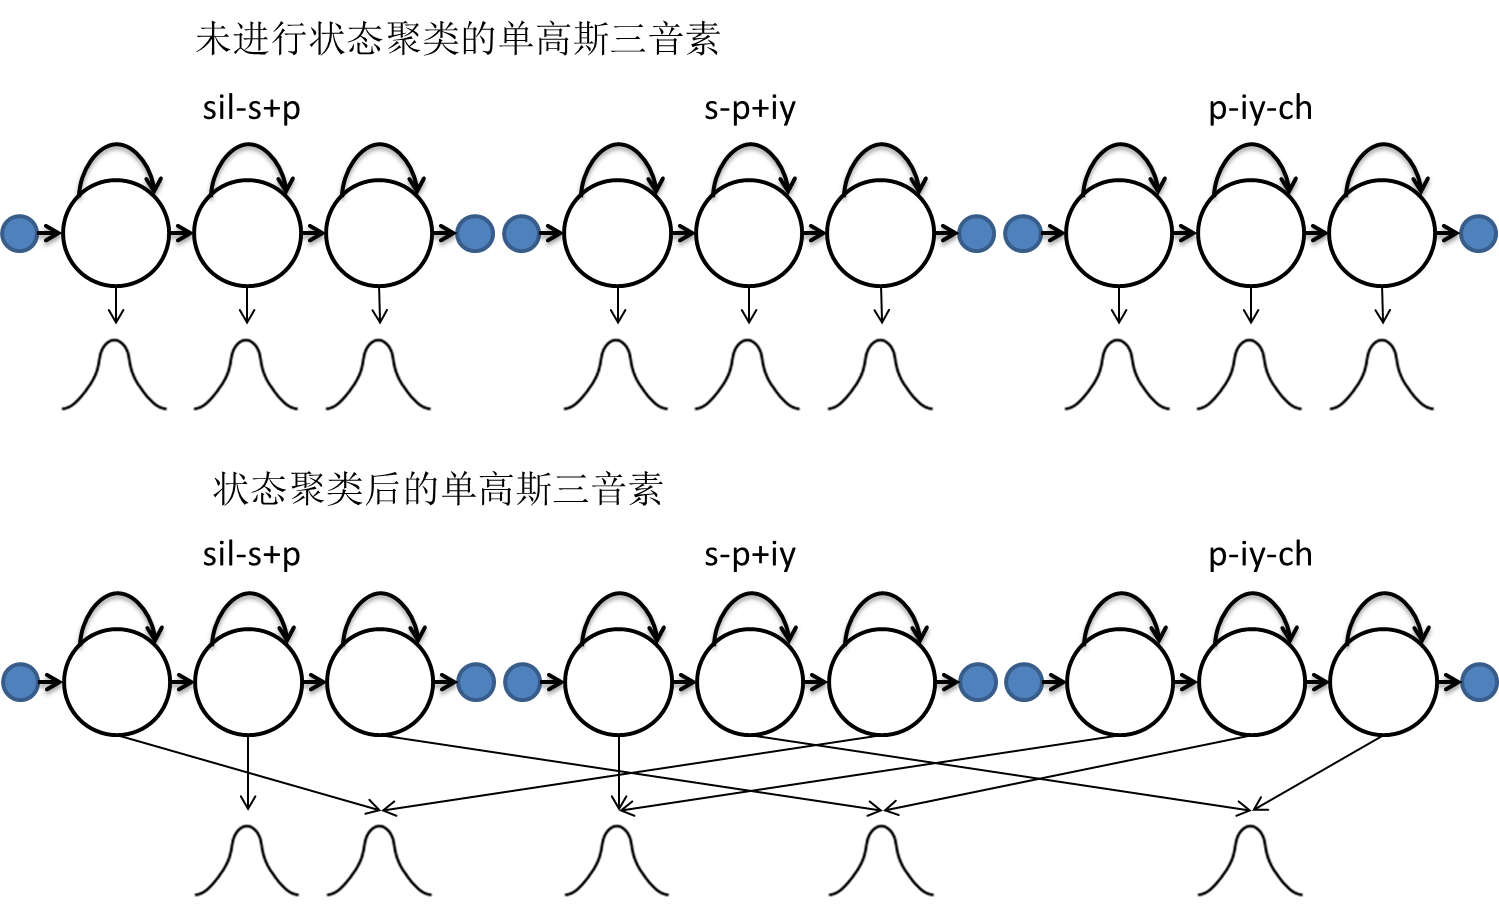
\includegraphics[width=.8\textwidth]{figure/state.png}
    \bicaption[fig:state-tying]{}{单高斯三音素的状态聚类}{Fig}{State clustering for single gaussian triphones}
\end{figure}

目前利用最广泛的聚类方法是基于数据驱动自底向上聚类。对训练集中存在的每一对语素之间计算一个距离,距离在某个阈值以内的语素将会被聚集在一起。数据驱动的主要问题在于当没有足够多训练数据时,这一方法将不再可靠,更严重的是,训练数据中不存在信息将无法被捕捉到。

另外一个更好的方法是利用音标决策树的方法来进行聚类。音标决策树是一棵包含了一系列关于每个音素左右上下文问题的二叉树,因为问题答案只有对和错。聚类自上而下开始,所有的状态都从根节点出发,通过回答上下文问题来分割左右儿子。直至处于当前节点的训练数据状态数目小于一个阈值,分割过程停止,此时叶子节点即为一个语素。决策树中的关键难题在于提问的顺序,目前最常用方法是在每次分裂时挑选能在分裂后似然增加的最大的那个问题。虽然这样决策树可能陷入局部最优,但它确实有效处理了对于不可见的三音素分类问题。

\subsection{语言模型}
\label{sec:lm}
语音模型建模的是候选标注的先验概率,假设候选标注含有$K$个单词,$\mathbf{w}=\{w_1, \dots, w_K\}$。通过条件概率公式,语音模型概率可以扩展为若干条件概率连乘:
\begin{equation}
    \label{eq:lm}
    P(\mathbf{w})=\prod_{k=1}^{K}P(w_k|w_{k-1}, ..., w_1)
\end{equation}
这里$w_k$是序列中的第$k$个单词。利用公式\ref{eq:lm}来计算先验概率需要记录整个句子的历史,然而在大词汇语音识别任务中,由于词表大小往往能达到10000词以上,所有可能的历史数据太过庞大,因此很难对每个可能的词序列都进行鲁棒估计。一种解决方案是限制历史的长度,N元组(n-gram)语音模型即利用了这一策略,它也是目前语音识别中最广泛利用的统计语言模型。它所作出假设是只需要最多利用N个单词作为历史就足够计算概率:
\begin{equation}
    P(w_k|w_{k-1}, ..., w_1) \approx P(w_k|w_{k-1}, ..., w_{k-N+1})
\end{equation}
这里$N$是预先定义的历史窗口大小,语音识别中通常利用$N=3$,也被称为三元语言模型。语言模型通常利用最大似然的准则进行训练,它的更新公式如下:
\begin{equation}
    P(w_k|w_{k-1}, ..., w_{k-N+1})=\frac{f(w_k,w_{k-1},...,w_{k-N+1})}{\sum_wf(w,w_{k-1},...,w_{k-N+1})}
\end{equation}
这里$f(w,w_{k-1},...,w_{k-N+1})$表示这$N$个词按顺序出现在训练数据中的个数。因为采用是最大似然估计,所以每个N-元序列得拥有充足的样本才能得到最鲁棒的估计。然而,即使$N$非常小,这一条件在大词汇连续语音识别任务中依然很难达成。所以,过去研究提出了若干平滑的方法来获得鲁棒的估计。
\begin{itemize}
    \item 降权(Discounting) \\
    降权方法用于解决训练集中未观测到N元组概率无定义的问题,它的主要思想是将被观测到的N元组概率乘上一个降权系数,将剩下的部分平均分配给未观测到N元组。最常用的降权方法有Good-Turing法~\cite{good1953population,katz1987estimation},Witten-Bell法~\cite{witten1991zero}和绝对降权法~\cite{ney1995estimation}
    \item 回溯法(Backing-off) \\
    回溯法利用训练数据中观测到的具有较短历史信息的词序列的组合概率来近似那些没有出现过、由较长历史信息组成词序列组合。
    \item 多模型插值(Interpolation) \\
    当一个N元语言模型不是很鲁棒时,可以通过和更低阶的语言模型进行插值以获得更平滑模型,比如在语音识别中通常会将单元,二元和三元语言模型进行插值来构建一个更鲁棒语言模型。插值的权重通常在一个校验集上调节得到。同样,我们也可以用同样的方法对由不同语料训练出N元语言模型进行插值。
\end{itemize}
语言模型训练和评价指标通常是困惑度(Perplexity, PPL),它定义是词序列生成概率的几何平均倒数:
\begin{equation}
    \text{PPL}=2^{-\frac{1}{K}\log(P(\mathbf{w}))}
\end{equation}
其中$K$是词序列包含的总词数,拥有更低PPL语言模型具有更低的不确定度和混淆度,通常也能潜在的降低语音识别词错误率。当然,这一关系并非一直成立,因而在语音识别中最终还是以词错误率来判断语言模型的好坏。

\subsection{解码及搜索}
\label{sec:decode}
如公式\ref{eq:asr}所示,解码的过程是在给定声学模型和语言模型之后寻找拥有最大概率路径。
\begin{eqnarray}
\mathbf{w}^* &=& \arg \max_{\mathbf{w} \in \mathcal{H}}p(\mathbf{O}|\mathbf{w})P(\mathbf{w}) \\
&=& \arg \max_{\mathbf{w} \in \mathcal{H}} \sum_{\mathbf{s}} P(\mathbf{s}|\mathbf{w})p(\mathbf{O}|\mathbf{s})P(\mathbf{w})
\end{eqnarray}
这里$\mathbf{s}$是所有可能的状态序列,$P(\mathbf{w})$通过语言模型计算,$P(\mathbf{s}|\mathbf{w})p(\mathbf{O}|\mathbf{s})$通过声学模型计算。正如我们在章节\ref{sec:calc_like}中讨论过的,这一似然可以通过前向后向算法进行计算。然而,因为候选词序列可能性过于庞大,无法通过对每个候选进行前向后向算法来计算似然。因此,实际中通常利用最大概率的状态路径来近似整个概率,即:
\begin{equation}
\label{eq:decode}
\mathbf{w}^* = \arg \max_{\mathbf{w} \in \mathcal{H}} \max_{\mathbf{s}} P(\mathbf{s}|\mathbf{w})p(\mathbf{O}|\mathbf{s})P(\mathbf{w})
\end{equation}
这样我们可以通过利用动态规划(Dynamic Programming, DP)的方法计算出拥有最大概率状态序列,然后以此推理出词序列,这一算法被称为Viterbi算法~\cite{viterbi1967error}。另$\phi_i(t)$表示在时刻$t$且输出了部分从$\mathbf{o}_1$至$\mathbf{o}_t$声学特征后停留在状态$i$的最大概率。它可以利用递归来计算:
\begin{equation}
    \phi_i(t)=\max_j\{\phi_j(t-1)a_{j,i}\}b_i(\mathbf{o}_t)
\end{equation}
这里$a_{i,j}$是状态转移概率,$b_i(\mathbf{o}_t)$是状态输出概率。最终:
\begin{equation}
    p(\mathbf{O}|\mathbf{w}) \approx \phi_{N}(T+1) = \max_i\{\phi_i(T)a_{i,N}\}
\end{equation}
Viterbi算法可以很容易扩展到连续语音识别,一种扩展后的Viterbi算法也被称为令牌传递(Token Passing)算法~\cite{young2002htk}。在这一算法中,每一个状态将不仅仅保留一个最优路径,而是保存若干个令牌。每一个令牌记录着某个候选词序列在第$t$时刻到达状态$i$的最优路径。在到达一个词边界时,语言模型的分数会直接加上。在整个观测序列结束时,拥有最大概率的令牌将被提取出来回溯其整个HMM序列。

即使利用了令牌传递算法,在大词汇连续语音识别中,传播所有令牌搜索代价依然十分庞大。为了减少计算代价,通常会利用基于集束搜索(beam search)剪枝方法。在这一方法中,所有$\phi_i(t)$低于$i$中最大概率减去一个阈值的令牌都会被移除,这一阈值也被称为集束(beam)宽度,剪枝也可以在加完语言模型之后进行。虽然beam搜索方法可以显著减少计算量,但是有可能在早期阶段利用了过窄的beam宽度而剪去了真正最优路径导致识别错误。所以,beam宽度设置需要在减少计算量和提升识别准确率之间进行均衡。

语言分数和声学分数之间动态范围的区别也是需要考虑问题,通常会分别对声学分数和语言分数进行缩放。另外需对插入错误添加额外惩罚,从而均衡词错误率中的插入和删除错误比例,因而最终语音识别中利用的准则是:
\begin{equation}
\mathbf{w}^* = \arg \max_{\mathbf{w} \in \mathcal{H}} \{\log p(\mathbf{O}|\mathbf{w}) + \alpha \log P(\mathbf{w}) + \beta L_{\mathbf{w}}\}
\end{equation}
这里$\alpha$是语言模型分数缩放系数,$\beta$是插入错误惩罚系数,$L_{\mathbf{w}}$是词序列长度。
通常会选择最大概率路径作为识别结果,也可以输出若干候选结果然后用更强的语言模型来重新评价(比如利用神经网络语言模型)。这一候选结果一般利用N-best列表~\cite{schwartz1990n}或者利用能包含更多信息词图(Word Graph/Word Lattice)~\cite{ortmanns1997word}。近些年来,基于加权有限状态机(Weighted Finite-State Transducer, WFST)~\cite{mohri2002weighted}的解码器被越来越多人采用,它的优点是可以将语言模型提前融合成一个网络,从而在解码时加快解码速度。




\section{大词汇连续语音识别中解码搜索技术}
\label{chap:intro-lvcsr}

语音识别既是一个模式识别问题,也包含相应的推理问题。前一个问题对各种语音、语言现象进行数学表示和描述,在基于统计学习的模式识别框架下进行建模,这决定了语音识别系统可达到识别精度的上限。而后一个问题在给定模型情况下,研究如何将输入语音和模型相匹配,推理得到最优识别结果,这决定了识别速度和实际可达的识别精度。
%
在语音识别的推理阶段,解码器功能是对声学模型计算出的声学特征概率和语言模型计算出的语言概率进行组合来得到最大概率的词序列。
%
在语音识别推理阶段,解码器是语音识别系统的核心和灵魂,所有信息都汇集于此。它将不同来源、 不同层次、 不同性质的知识和信息关联在一起,使它们互相之间取长补短, 从而得到正确的语音识别结果。因此,如何将各种性质相异信息有机融合是解码网络和解码算法设计中必须认真研究和解决的问题。
从解码器的作用来看,它既是语音识别研究中验证各种理论、模型、算法
正确性的基本实验平台,也是构建实用系统的基础。因此,在解码器设计中也
需要兼顾研究的方便与工程实际应用。

\subsection{解码器的技术流派}
\label{chap:intro-lvcsr-decmethod}

根据前面章节讨论,一个完整的语音识别系统包含了自底向上的五层映射关系:
语音观测到 HMM 状态、 HMM 状态到上下文相关音素、上下文相关音素到音素、
音素到词、词到句子。
具体来说公式~\ref{eq:decode}可以进一步展开如下:
\begin{equation}
 \begin{split}
\mathbf{w}^* = \arg \max_{\mathbf{w} \in \mathcal{H}} \max_{\mathbf{s}} P(\mathbf{s}|\mathbf{w})p(\mathbf{O}|\mathbf{s})P(\mathbf{w}) \\
= \arg \max_{\mathbf{w}} \sum_{\mathbf{l}} \sum_{\mathbf{c}} \sum_{\mathbf{s}}
p(\mathbf{O}|\mathbf{s}) \cdot
P(\mathbf{s}|\mathbf{c})\cdot P(\mathbf{c}|\mathbf{l})\cdot P(\mathbf{l}|\mathbf{w}) \cdot 
P(\mathbf{w})
 \end{split}
\end{equation}
其中展开后式子每一项分别对应上述的五层映射关系。
语音观测无法在识别之前得知,因此语音观测到 HMM 状
态的映射需要在解码过程中动态建立,对应声学分数也需要实时计算。
对于 HMM 状态到上下文相关音素、上下文相关音素到音素、音素到词这三层映
射关系,一旦发音字典、声学模型确定便不再改变。出于对解码效率的追求,人
们通常把它们静态地编译到解码网络中去。对于没有任何约束的大词汇连续语音识别任务而言,
词可以以任意方式组织成句, 故而从原理上讲, 词、 句间映射关系只能在解码
过程中动态建立。 但是由于表征词与词之间关联度(概率)的 N 元文法模型在解
码前便已存在且是一个有限集合, 所以在实际中, 语言模型分数计算却可
以用不同的方式实现。 在语音识别领域,通常根据解码器中语言模型的表示、 语
言模型状态获取以及语言模型分数计算方法的不同把解码器分为两大流派:
\begin{itemize}
\item 动态网络解码器: 在动态网络解码器中,解码网络仅包含发音字典和声学
模型,不含有语言模型任何信息。 语言模型状态在解码过程中随着词与词相连
成句而动态地生成、语言模型分数通过查表的方式动态获取。这类解码器的典型
代表是基于发音前缀树(Pronunciation Prefix Tree, PPT)~\cite{woodland1994large}网络解码器。
\item 静态网络解码器: 在静态网络解码器中,解码网络不仅包含发音字典和声
学模型,也包含完整的语言模型。 语言模型状态以及状态转移以有限状态机的形
式合成进解码网络中去, 语言模型分数则作为状态转移概率存储于边上。解码时,
仅需逐边积累整条路径状态转移概率便可获得语言模型分数。这类解码器的典
型代表是基于加权有限状态转换器(WFST)~\cite{mohri2002weighted}的解码器。
\end{itemize}

静态网络解码器作为一种以空间换时间策略,通过精心的优化,一般可以
获得更快的识别速度, 但是其缺点也是显而易见,即:构建的解码网络规模过
大,尤其是在采用高阶语言模型和声学模型情况下,由于内存大小限制,要
将所有的知识源都编译进解码网络中往往是不可行。因此,近年来基于动态解
码网络传统语音识别方法又逐渐受研究人员青睐~\cite{soltau2009dynamic,rybach2011comparative}, 能够几乎不受任何约束
地利用高阶语言模型和声学模型以便获得更优的识别精度, 应用面更广, 这是动
态网络解码器最为诱人之处。然而动态网络解码器的设计和束搜索剪枝方法更为
复杂,需要调整参数和门限更多,挑战性更大。 

除了从解码网络的结构上进行分类,还可以根据搜索最优路径不同方式,
将解码器分为时间异步搜索解码器和时间同步搜索解码器:

\begin{itemize}
\item 时间异步搜索解码器: 在较老的解码器,例如: IBM ViaVoice 中, 采用深
度优先方式在解码网络中搜索最优词序列, 是一种时间异步搜索。由于这类解码
器在解码过程中需要用到若干后进先出的缓冲区(即:堆栈)来保存扩展得到
词识别假设,所以也常常被称为堆栈解码器(Stack decoder)~\cite{paul1992efficient}。 
与时间同步搜索相比,其好处在于:通过选取适当启发式函数(Heuristic function),可以将搜
索局限于最优路径附近,提高搜索效率。 但这也造成了它的主要缺陷: 1) 启发式
函数要综合声学和语言两方面分数,有时还需要“将来”路径的信息, 因此非
常难以获得; 2)由于是时间异步搜索,所以搜索过程中产生路径长度各不相同,
使得剪枝难于实现。因此,目前堆栈解码已很少用于直接对语音观测进行解码,
而是更多地作为一种后处理手段, 用于从词图中生成 N-Best 结果。
\item 时间同步搜索解码器:时间同步搜索是目前解码器设计与实现中主流方
法,又称帧同步搜索。它采用广度优先方式从解码网络中找出与输入特征序列最
匹配的状态序列,从而得到相应的最优音素序列和词序列。这一类解码器通常采
用 Viterbi 算法或是令牌传递(Token passing)算法~\cite{woodland1994large}实现。 
\end{itemize}

解码器不仅算法复杂,并且实现起来需要较高工程化能力和技巧, 在开发
完成后也往往需要不小人力和时间才能够调优, 因此各个研究机构与商业公司
都对自己解码器的实现细节讳莫如深。 尽管如此,目前世界上还是存在一些以学
术研究为目的开源解码器可以作为研究的基础, 表
列出了其中较为知名。这些解码器的网络结构和解码算法各异,但由于是以学术研究为目的,因此速度
优化方面大部分较差。


\begin{table}[thbp!]
  \caption{\label{tab:perf-compare} {\it  知名开源解码器 } }
  \centerline{
    \begin{tabular}{c c  c c}
      \toprule
      解码器 &  研发机构 & 网络结构 & 搜索算法 \\
      \midrule
      HDecode & 英国剑桥大学 & 动态,发音前缀树 & 单遍, 令牌传递 \\
        Sphinx &美国卡内基梅隆大学 &动态,发音前缀树 &单遍, 令牌传递 \\
        RASR &德国亚琛工业大学& 动态, 发音前缀树 &单遍, Viterbi \\
        Juilus & 日本京都大学 & 动态, 发音前缀树 & 两遍, 前后向搜索。\\
        Juicer & 瑞士IDIAP & 静态, WFST & 单遍,令牌传递 \\
        Kaldi & 美国约翰霍普金斯大学 & 静态, WFST & 两遍,令牌传递     \\
\bottomrule
    \end{tabular}
  }
\end{table}

多遍搜索与单遍搜索(1-pass)相比各有优劣,在实际中也都有应用。多遍搜
索的拥护者认为: 通过第一遍粗搜索可以大大缩小解码空间, 使得在后续解码过
程中利用更加精细语言模型和声学模型成为可能,避免了单遍解码器中的时间、
空间约束问题。单遍搜索的拥护者认为多遍解码有三个主要问题: 1) 由于第二遍
解码必须等待第一遍解码完成,所以多遍搜索很难应用于实时解码。 2) 每一遍解
码都会引入不可恢复剪枝错误,这些错误不论在后续解码中采用何种模型都无
法弥补。要解决这一问题还是得在单遍搜索算法上下功夫,与其这样,还不如直
接做好单遍解码器。 3) 多遍解码器的每一遍解码采用的特征、声学模型、语言模
型、搜索算法都不尽相同。

\subsection{结构和主要模块}
\label{chap:intro-lvcsr-decmodule}

\subsubsection{解码器框架}

图~\ref{fig:dec_arch}给出了典型解码器结构。不论是哪种类型解码器通常都包含网络生
成、分数计算、搜索、剪技与路径管理这五部分,它们的功能逐一介绍如下。

\begin{figure}[!htp]
  \centering
    \captionstyle{\centering}
    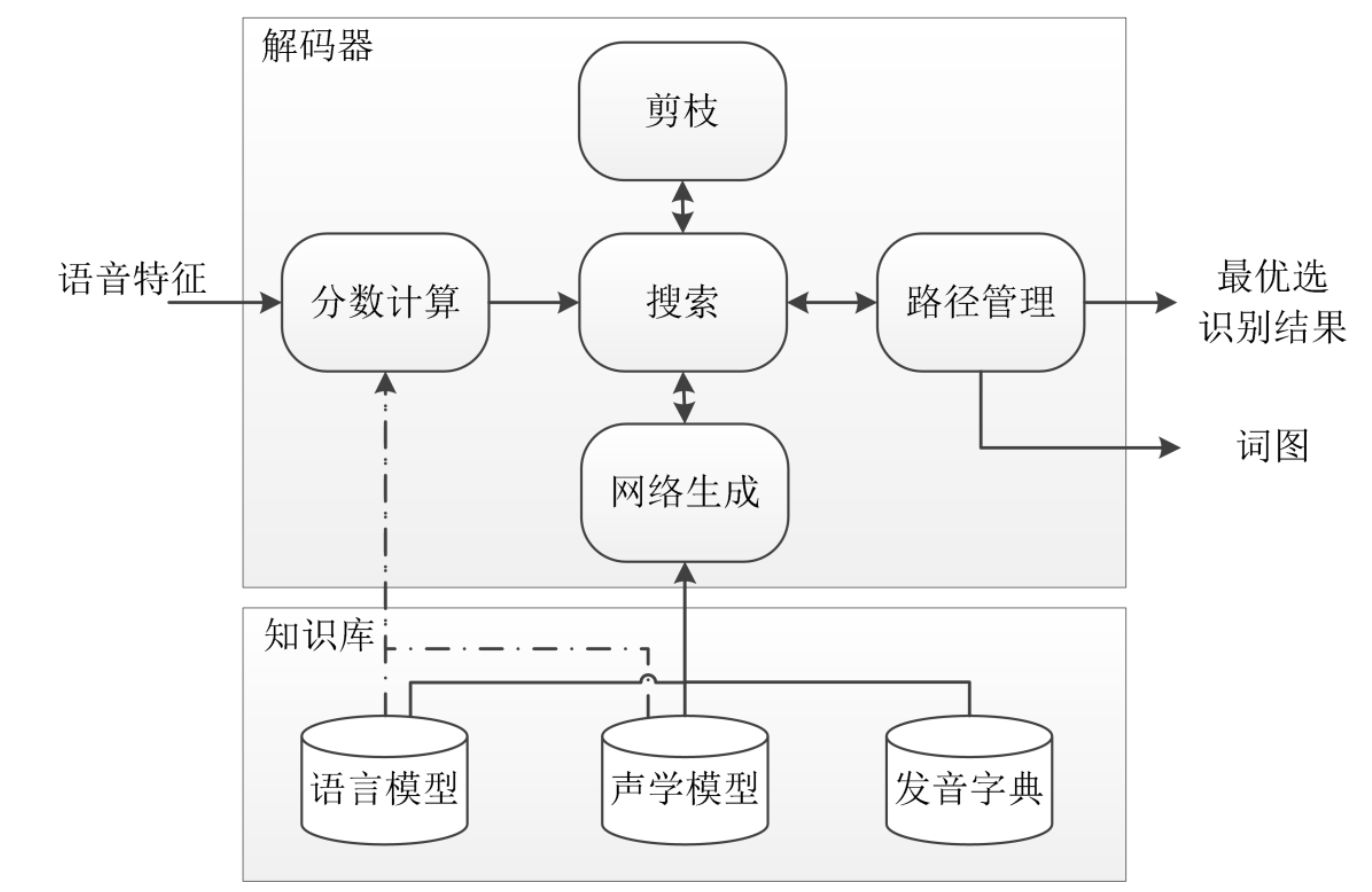
\includegraphics[clip=true, width=.9\textwidth]{figure/dec_arch.png}
    \bicaption[fig:dec_arch]{}{通用解码器架构}{Fig}{General Architecture of ASR Decoder}
\end{figure}


\subsubsection{网络生成}

网络生成模块主要负责将构建解码搜索空间。搜索空间,又称解码网络, 一般以音素 HMM 或 HMM 状态连缀而成,由语言模型、发音字典、声学模型和其
他相关知识源编译而来。
大词汇连续语音识别系统解码网络是由各个知识源构成一个搜索空
间,一般来讲可以分为动态构建的解码网络和静态网络。基于动态网络的解码
器,以前缀树发音词典作为搜索网络,语言模型则通过动态查询方式把得
分引入解码过程之中,然后利用重入字典树或者字典树拷贝的方式对整个解
码网络进行搜索~\cite{young2002htk}。动态网络解码器优势在于,由于字典和语言模型是分
离,其占用内存较少,这个特点在以往移动网络技术和硬件技术不发达的时
期,尤其是在嵌入式设备上内置解码器的时代占有绝对优势,这是由嵌入设备
硬件条件决定的。但是动态网络的缺点是它时间复杂度较高、解码速度较
慢,这也使其越来越难以满足当前海量语音识别需求。随着移动互联网
和嵌入式设备的普及以及云技术发展,语音识别应用发展为在嵌入式设备
上仅仅保留简单的前端,而识别系统保留在服务器云端。这时基于加权有限状
态机的静态网络解码器快速优势就体现出来了,更短的识别时间能让服务器
在单位时间内接受更多识别任务,因此静态编译的解码网络更适合用于海量
的语音识别任务。

在 LVCSR 任务中,解码网络通常非常庞大,因此网络生
成过程中需采用多种手段对网络结构进行优化,在不改变网络功能前提下,尽
可能地减少网络中节点和边的数目。 解码网络是解码器基础,决定了解码器
其他部分应当采用何种方法实现。在静态网络解码器中,解码网络不仅包含发音字典和声
学模型,也包含完整的语言模型。 语言模型状态以及状态转移以有限状态机形
式合成进解码网络中去, 语言模型分数则作为状态转移概率存储于边上。解码时,
仅需逐边积累整条路径状态转移概率便可获得语言模型分数。这类解码器的典
型代表是基于加权有限状态转换器(WFST~\cite{mohri2002weighted}的解码器。

加权有限状态机最开始是由AT\&T实验室Mohri和Riley等人在1997年引
入语音识别领域的。并且在理论上发展了确定化、最小化等一系列网络优化算
法,为语音识别的应用打好了理论基础。语音识别各模型组件分别用如下方式进行WFST构建:

\begin{itemize}
\item N元语言模型在WFST中被表示为G。从N元语言模型的含义可知,它提供的是当前词对于词历史
概率。语言模型需要有信息记录其至多N个词的历史。但是,WFST应用在语音
识别时是不允许输入输出带有串的(即输入输出都是其符号集单个元素)。
因此不能用G构造过程的输入输出上表示其历史,而应选用在状态上记录历史。
另外一个问题是N元语言模型的回退(Back-off),当语言模型训练语料
未出现某一个N元词组的时候,就会以一个回退的(N-1)元模型概率乘以一个
系数来替换。这部分表示为一个带有权重空输入的状态跳转边。

\item 字典在WFST中被表示为L。
字典其实是对发音规则的一种表示,最简单方法就是在开始状态和结尾
状态之间列出每个词的发音。同时,由于在和语言模型合成的时候,词与词是
相连,不能够到达终止状态就完结了,需要用一个空边从终止状态连接到开
始状态形成一个闭环。
针对字典的同发音问题,Mohri在文献~\cite{mohri2002weighted}中提出对于不同词的同发音发音
序列加入一组辅助符号,这样对于同发音词,其环路的输入
符号就不再相同,可以确保字典的可确定化。

\item 上下文相关声学模在WFST中被表示为C。
一个上下文相关triphone模型一般表示为a-b+c,其中b是中心音素,
a和c为其前后上下文音素~\cite{seide2011conversational}。用WFST表示triphone模型实际上是把三音素
和单个的音素进行对应,其输出就和发音字典的输入相互对应,由此可以进行进一步合成。

\item 隐马尔可夫模型在WFST中被表示为H。
隐马尔可夫模型天然具有多个状态跳转特性,因此可以直接将其构建为多个WFST状态。隐马尔科夫模型的转移概率被转化为WFST的权重。而WFST输入是隐马尔科夫模型的状态编号,输出是该隐马尔科夫模型所表示的triphone建模单元。
\end{itemize}

当各个知识源WFST组件被构建完毕以后,可以利用WFST合成和优化算法将各组件最后进行合并。如下:
\begin{equation}
HCLG = min(det(H \circ min(det(C \circ min(det(L \circ G))))))
\end{equation}

最终生成的WFST包含了所有的知识源,后文所讨论维特比搜索就在它上面进行。

\subsubsection{分数计算}

分数计算模块计算输入特征序列声学和语言分数, 提供给搜索模块利用。
应当计算何种分数与解码网络结构和搜索算法有关。例如,在静态网络解码器中,
语言模型分数已编译于解码网络之中,所以只需要计算声学分数即可;而对于动
态网络解码器, 除声学分数外, 还需要计算语言模型分数。 在分数计算方面研
究主要集中于如何实现分数的快速计算, 对于声学分数通常从如下三个方面进行:

\begin{itemize}
\item 硬件加速。利用 CPU 矢量计算器~\cite{kanthak2000using}
或通用图形处理器(Graphics
Processing Unit, GPU)~\cite{chong2009fully}
加速分数计算。这类方法通常不会带来计算误
差(与硬件实现相关),所以对识别精度没有影响。
\item 模型简化。采用复杂度更小、参数更少的模型,或通过聚类和参数共享减
小模型复杂度。例如采用半连续 HMM~\cite{huang1990semi} 替代连续 HMM,以及传统参数共享方法~\cite{young2002htk}亦属此类。这类算法一般都会带来识别精度损失,所以需要在
识别精度、模型复杂度和计算速度之间做好权衡。
\item 算法优化。 对声学分数的计算过程进行简化。这类方法一般是对声学分数
进行近似计算,所以必然会带来一定识别精度损失。一般而言, 衡量一个近似
算法是否可用的标准是看其带来相对识别精度损失是否可控制在5\%以内~\cite{cai2009efficient}。
\end{itemize}

对于语言分数计算,当采用 N 元文法模型时,通常从两个途径进行加速: 1)
减小每次查表操作耗时,典型方法是采用最小完美哈希(Minimal Perfect Hash,
MPH)表实现语言模型的存储与检索~\cite{li2007fast,cardenal2002fast}; 2) 引入分数缓存~\cite{huijbregts2008fast}减少查表次数。

\subsubsection{维特比搜索}

搜索模块负责在解码网络上搜索得到最优路径。不论是静态还是动态网络解
码器,目前都以令牌传递算法~\cite{young1989token}为主流的搜索算法。

令牌传递是 Viterbi 算法另一种更为普遍和简便的实现形式。 在该算法中,
每一个 HMM 状态都可以关联一个令牌(Token),令牌中存储着到当前帧为止该
令牌所经历历史路径和路径分数。解码是把令牌从解码网络初始状态按照状
态转移的约束(即:沿解码网络的边) 向终止状态传递过程。每一帧令牌向前
传递一次,传递同时更新令牌分数与路径信息,并在多个令牌同时传递到一个
状态上时进行令牌合并——只保留分数最高的令牌。在所有帧都处理完成后,即
可得到最优路径和最优路径分数。

令牌传递算法的优点是可以方便地在令牌上附着其他信息以便在状态节点之
间传递,从而实现更复杂解码过程,例如: 为了生成词图,在令牌合并时, 不
是将次优令牌丢弃,而是作为其他候选路径附于合并后的令牌之上。

\subsubsection{剪枝}

LVCSR 中,搜索空间的过于庞大使得对整个解码网络进行全搜索不可能实现,
剪枝用于在解码过程中把分数过低路径剔除,从而达到降低计算量,同时保证
识别性能基本不降目的。根据解码器不同,剪枝可应用于搜索的各个阶段(如:
词首或词尾), 或是各个层次(如:词级、音素级、状态级、令牌级), 但都可
归纳为两种基本方式:
\begin{itemize}
\item 束剪枝(Beam pruning) :束剪枝保留与最优路径分数较近的次优路径。
令 $v(t,j)$ 表示第 t 帧位于状态 j 最优路径分数,则第t 帧的最优路径分数为:
\begin{equation}
v_{max}(t)=max_s v(t,s)
\end{equation}

令 $f$ 为剪枝门限(又称为束宽),则束剪枝只保留所有满足下式的路径:
$v(t,j)>v_{max}(t)\cdot f$
\item 直方图剪枝(Histogram pruning) :与束剪枝不同,直方图剪枝仅保留分
数最高 N 条路径, N 为设定剪枝门限。之所以称为直方图剪枝是因为该方法
可以采用直方图统计高效地实现~\cite{pylkkonen2005new}。
\end{itemize}

\subsubsection{路径管理和词图}

路径管理模型主要作用是对搜索过程中得到的路径链表进行回溯,生成 1-Best、
N-Best 结果和词图。同时,它也负责对剪枝过程中剪掉的“垃圾”路径进行内存
回收等操作。

\begin{figure}[!htp]
  \centering
    \captionstyle{\centering}
    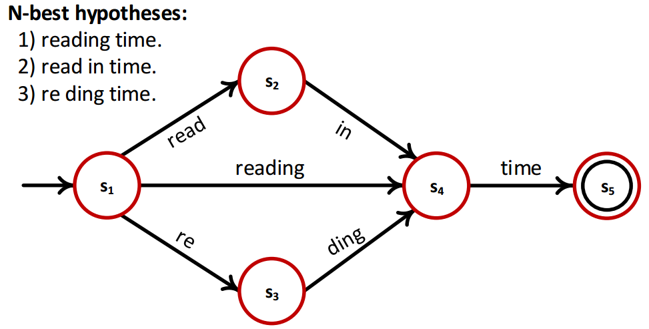
\includegraphics[clip=true, width=0.6\textwidth]{figure/lattice.png}
    \bicaption[fig:lattice]{}{N-Best候选序列和词图}{Fig}{N-Best Hypothesis and Lattices}
\end{figure}


由于N-Best候选序列中往往存在大量公共部分(比如图~\ref{fig:lattice}中的“time”这个词),因此将公共部分压缩在一起进行表示,也就是将多个候选序列转换成一张图来进行存储,将会更加高效。在语音识别中,这样一张图就称为词图。词图的生成所带来的额外操作与生成N-Best候选序列类似。具体来说,其往往要求在解码过程中做令牌合并时,保留多个历史记录。在记录完词图后,还需要词图剪枝步骤,其将冗余和无法连通边和结点删去,得到最终比较紧致的词图。

词图具有较多用途(一些例子如图~\ref{fig:lattice-usage}所示),因此相较于N-Best候选序列,词图的处理往往是语音识别系统中的一个标准模块。

\begin{figure}[!htp]
  \centering
    \captionstyle{\centering}
    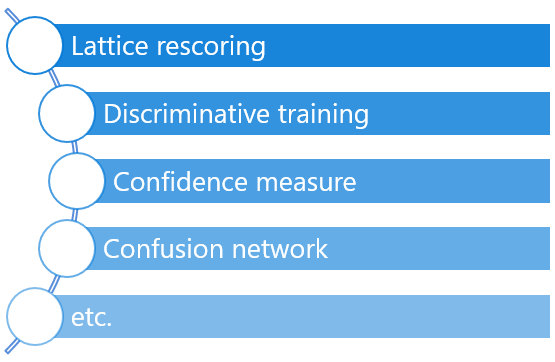
\includegraphics[clip=true, width=0.4\textwidth]{figure/lattice_usage.png}
    \bicaption[fig:lattice-usage]{}{词图用途举例}{Fig}{Applications of Lattices in ASR}
\end{figure}


\section{本章小结}
\label{chap:intro-sum}

在这章中我们简要介绍了语音识别的基本内容,首先讨论了特征提取,包括MFCC,PLP,FBANK等三种语音识别中常用特征;接着介绍了语音识别中最成功的声学模型——HMM以及利用最大似然估计和序列鉴别性准则来优化HMM模型;继而讨论了现实语音识别系统中的声学单元和参数绑定;最后讨论了N元语言模型和Viterbi解码等内容。

同时,本章回顾了语音识别推理阶段搜素解码部分基本内容和方法。
解码器对声学模型计算出的声学特征概率和语言模型计算出的语言概率进行组合来得到最大概率词序列。
%
在语音识别推理阶段,解码器是语音识别系统核心和灵魂,所有的信息都汇集于此。它将不同来源、 不同层次、 不同性质的知识和信息关联在一起,使它们互相之间取长补短, 从而得到正确语音识别结果。因此,如何将各种性质相异信息有机融合是解码网络和解码算法设计中必须认真研究和解决问题。
从解码器的作用来看,它既是语音识别研究中验证各种理论、模型、算法的
正确性的基本实验平台,也是构建实用系统的基础。因此,在解码器的设计中也
需要兼顾研究的方便与工程实际应用。